\documentclass{article}
\usepackage{neurips_pa}
\usepackage{graphicx,booktabs,amsmath,amssymb,xcolor,caption}
\usepackage[hidelinks]{hyperref}
\captionsetup{font=small,labelfont=bf,skip=3pt}
\setlength{\textfloatsep}{8pt plus 2pt minus 2pt}
\setlength{\floatsep}{6pt plus 2pt minus 2pt}
\setlength{\intextsep}{6pt plus 2pt minus 2pt}
\newcommand{\pp}{\,pp}
\newcommand{\TaRcA}{98.4}
\newcommand{\TaRcF}{98.4}
\newcommand{\TaRcP}{0.95}
\newcommand{\TaRgD}{$-1.8$}
\newcommand{\TaRgC}{96.2}
\newcommand{\TaRhD}{$-3.8$}
\newcommand{\TaRhC}{95.4}
\newcommand{\TaRsD}{$-9.6$}
\newcommand{\TaRsC}{89.6}
\newcommand{\TaRsW}{0.68}
\newcommand{\TcRs}{129}
\newcommand{\TcRt}{58}
\newcommand{\TcRo}{138}
\newcommand{\TcRb}{69.0}
\newcommand{\TcRc}{57.5}
\newcommand{\TcRbc}{70.1}
\newcommand{\TaVcA}{98.0}
\newcommand{\TaVcF}{98.0}
\newcommand{\TaVcP}{0.96}
\newcommand{\TaVgD}{$-1.8$}
\newcommand{\TaVgC}{95.8}
\newcommand{\TaVhD}{$-2.0$}
\newcommand{\TaVhC}{96.6}
\newcommand{\TaVsD}{$-6.0$}
\newcommand{\TaVsC}{91.6}
\newcommand{\TaVsW}{0.51}
\newcommand{\TcVs}{191}
\newcommand{\TcVt}{29}
\newcommand{\TcVo}{105}
\newcommand{\TcVb}{86.8}
\newcommand{\TcVc}{67.7}
\newcommand{\TcVbc}{86.8}
\newcommand{\TaCcA}{97.4}
\newcommand{\TaCcF}{97.4}
\newcommand{\TaCcP}{0.14}
\newcommand{\TaCgD}{$-2.8$}
\newcommand{\TaCgC}{95.2}
\newcommand{\TaChD}{$-2.8$}
\newcommand{\TaChC}{94.0}
\newcommand{\TaCsD}{$-20.6$}
\newcommand{\TaCsC}{77.0}
\newcommand{\TaCsW}{0.11}
\newcommand{\TcCs}{220}
\newcommand{\TcCt}{24}
\newcommand{\TcCo}{81}
\newcommand{\TcCb}{90.2}
\newcommand{\TcCc}{75.1}
\newcommand{\TcCbc}{90.1}
\newcommand{\TaZcA}{94.8}
\newcommand{\TaZcF}{94.6}
\newcommand{\TaZcP}{0.93}
\newcommand{\TaZgD}{$-1.8$}
\newcommand{\TaZgC}{94.8}
\newcommand{\TaZhD}{$-1.6$}
\newcommand{\TaZhC}{94.6}
\newcommand{\TaZsD}{$-14.4$}
\newcommand{\TaZsC}{80.2}
\newcommand{\TaZsW}{0.56}
\newcommand{\TcZs}{228}
\newcommand{\TcZt}{17}
\newcommand{\TcZo}{80}
\newcommand{\TcZb}{93.1}
\newcommand{\TcZc}{75.4}
\newcommand{\TcZbc}{93.8}
\newcommand{\TcN}{325}
\newcommand{\TcRej}{0}
\newcommand{\TrepRows}{Grayscale & 0.808 & 0.81 / 0.69 & 96.2 & 0.741 & 0.75 / 0.58 & 95.8 & 0.889 & 0.89 / 0.85 & 95.2 \\
Hue $+108^\circ$ & 0.755 & 0.76 / 0.60 & 95.4 & 0.712 & 0.72 / 0.57 & 96.6 & 0.884 & 0.89 / 0.85 & 94.0 \\
Shift 8\,px & 0.967 & 0.97 / 0.95 & 98.7 & 0.945 & 0.95 / 0.91 & 98.7 & 0.977 & 0.98 / 0.96 & 97.0 \\
Shift 32\,px & 0.929 & 0.93 / 0.91 & 97.9 & 0.943 & 0.94 / 0.87 & 98.7 & 0.965 & 0.97 / 0.94 & 96.9 \\
Patch shuffle & 0.694 & 0.70 / 0.66 & 89.6 & 0.635 & 0.64 / 0.58 & 91.6 & 0.755 & 0.76 / 0.73 & 77.0 \\
Cue conflict & 0.313 & 0.47 / 0.21 & 40.0 & 0.322 & 0.45 / 0.14 & 58.8 & 0.711 & 0.74 / 0.66 & 67.7 \\}


\title{Beyond the IID Comfort Zone: Shortcuts, Shifts,\\ and Knowing When to Say ``I Don't Know''}
\author{Ahmed Waqas \\ Roll No.\ 27100150 \\ LUMS -- Advanced Topics in Machine Learning, PA1}

\begin{document}
\maketitle

\begin{abstract}
In this report, we inspect how deep learning models react to real-world situations where the test data thrown at a model doesn't match the data it was trained on, or where the model is forced to deal with completely unknown classes. Across four controlled tasks, we test how different architectures, training methods and access to target data change what a model actually learns. In our first task, we look at the built-in biases of ResNet, ViT and CLIP. By altering the images (removing colour, swapping textures, shifting and shuffling patches), we expose whether these models are really looking at global shapes or just taking shortcuts through local texture and other cues. Second, we test unsupervised domain adaptation on PACS, with sketches as the unlabeled target. We show that blindly forcing domains to look identical (DANN) can break training and cause negative transfer (worse performance than the source-only baseline). We expected aligning specific classes, like matching photo dogs with sketch dogs (CDAN), to fix this, but in our runs it made things much worse, and only the simplest alignment (DAN) gave a small gain. Third, we test domain generalization, where unlike UDA the target domain is completely hidden during training. We compare a standard baseline against methods that try to wipe out domain differences (DAN-DG) or find stable, flat areas in the loss landscape (SAM) to see what actually helps a model survive an unseen domain. Finally, we perform open-set recognition on CIFAR to see whether our models can safely tell apart images they know from ones they don't, comparing simple post-hoc scoring methods against a technique that actively prepares the model for unknowns (PROSER).
Putting it all together, this report looks at the balancing act of building robust models: we want them to ignore surface-level domain shifts, keep the features that actually separate classes, and avoid making overconfident guesses on novel inputs. Code, configs, splits and all result files: \url{https://github.com/ahmedmahni07-commits/27100150_PA1}.
\end{abstract}

\section{Introduction and research questions}
Standard machine learning operates on a very generous assumption: that the data a model sees in the real world will look exactly like the data it was trained on (the IID assumption). In the real world, this assumption completely falls apart. For instance, if you take a predictive maintenance model trained on vibration data from one specific 3-phase induction motor and apply it to a different machine on the factory floor, the background noise changes, operating conditions shift, and completely novel faults might appear. The real world doesn't care about our training distributions. This report explores exactly what happens when models are pushed beyond their closed-set, IID comfort zones.

We start by asking what a model is actually looking at when it gets an image right. In Task~1 we take ResNet, ViT and CLIP and feed them heavily altered images, to see whether they have genuinely learned the global shape of an object or are taking lazy shortcuts through local texture, colour or layout, and whether their internal features change even when their predictions don't. Task~2 moves to domain shift. If we have labeled photos, paintings and cartoons plus a pile of unlabeled sketches, can we force a model to bridge the gap by aligning the domains in feature space, and what happens when that alignment is done blindly? Task~3 makes the problem harder by hiding the sketches completely during training, and compares plain training against removing differences between the source domains and against searching for flat, stable minima. Finally, Task~4 deals with the fact that a normal classifier must always pick one of its known labels, even for an object it has never seen. There we try to make a model say ``I don't know'' to near and far unknowns, comparing simple scores computed on a trained model against a method that reserves space for unknowns during training. All four tasks feed into one question, which we return to in Section~\ref{sec:disc}: \emph{what should a robust representation keep, what should it learn to ignore, and when should it refuse to predict?}

%==========================================================================
\section{Experimental setup}\label{sec:setup}
All runs use seed 6304, and each hypothesis and metric was fixed before looking at the result.

\paragraph{Task 1.} We use STL-10 and three frozen backbones: ResNet-50 and ViT-B/16 (both trained on ImageNet) and CLIP ViT-B/32. On top of each we train a simple linear classifier on 80\% of the training set, keeping the best checkpoint on the remaining 20\%. CLIP is also tested zero-shot using the prompt ``a photo of a \{class\}.'' Everything is evaluated on the same 500 test images (50 per class), and every change is applied to the same $224{\times}224$ image, so all models see exactly the same pixels. For colour we test grayscale and a hue rotation of about $108^\circ$, which keeps brightness, edges and texture but changes every colour. We expected hue rotation to hurt more than grayscale. For shape vs.\ texture we build cue-conflict images with AdaIN style transfer, taking the shape from one class and the texture from another, across five class pairs (dog vs.\ car, cat vs.\ truck, bird vs.\ airplane, horse vs.\ ship, monkey vs.\ deer) in both directions. We expected ResNet to follow texture the most and CLIP to follow shape the most, and we report shape bias together with coverage (how often the model picks either of the two intended classes). For spatial structure we shift each image by 8, 16 and 32\,px in four directions, and separately cut it into a $4{\times}4$ grid and shuffle the tiles. We also measure how far each backbone's features move (cosine similarity $I_T$) and plot them with t-SNE.

\paragraph{Tasks 2 and 3.} Both use PACS with Photo, Art Painting and Cartoon as labeled sources and Sketch as the target. We fine-tune a full ImageNet ResNet-18 with a 7-class head and pick checkpoints using only the average validation F1 on the three source domains, never Sketch. In Task~2 the adaptation methods also see unlabeled sketches: DAN adds a penalty on the statistical distance (MMD) between source and sketch features; DANN adds a domain classifier that the network is trained to fool; and CDAN does the same while also giving the domain classifier the model's class predictions. In Task~3 sketches are never seen. ERM is simply the Task~2 source-only model, DAN-DG applies the same MMD penalty between each pair of source domains, and SAM trains towards flat minima. As diagnostics we report \emph{domain separability}, the accuracy of a simple classifier trained to tell domains apart from the frozen features (50\% is chance in Task~2 and 33\% in Task~3), and a \emph{sharpness} score, the rise in loss after a small step in the worst direction. DANN diverged when implemented exactly as specified, so for DANN and CDAN we added gradient clipping and normalised the domain classifier's input.

\paragraph{Task 4.} We train a CIFAR-style ResNet-18 from scratch on CIFAR-10 (100 epochs, keeping the best validation checkpoint). GCSC is the same model with stronger RandAugment augmentation. PROSER starts from that model and fine-tunes it for 50 epochs with five extra ``dummy'' outputs, which learn to fire on mixtures of two different known classes. The unknowns are 800 near images (e.g.\ wolf, bus, pickup truck) and 800 far images (e.g.\ keyboard, bowl, wardrobe) from CIFAR-100, used only for the final evaluation. We score unknownness in four ways: low softmax confidence (MSP), low maximum logit (MLS), energy, and Mahalanobis distance to the class centres. Each threshold is set so that 95\% of CIFAR-10 validation images are accepted.

%==========================================================================
\section{Results}
\subsection{Task 1: what are the models actually looking at?}

\begin{table}[t]
\centering\small
\caption{Clean baseline and pixel interventions on the 500-image STL-10 subset. Acc.\ and F1 are in \%. Cons.\ is the \% of predictions that stay the same as on the clean image; MaxP is the average confidence; MaxP$_\text{wrong}$ is the average confidence on shuffled images the model gets wrong.}
\label{tab:t1}
\setlength{\tabcolsep}{3.2pt}
\begin{tabular}{l ccc cc cc ccc}
\toprule
 & \multicolumn{3}{c}{Clean} & \multicolumn{2}{c}{Grayscale} & \multicolumn{2}{c}{Hue $+108^\circ$} & \multicolumn{3}{c}{Patch shuffle $4{\times}4$}\\
\cmidrule(lr){2-4}\cmidrule(lr){5-6}\cmidrule(lr){7-8}\cmidrule(lr){9-11}
Model & Acc & F1 & MaxP & $\Delta$Acc & Cons. & $\Delta$Acc & Cons. & $\Delta$Acc & Cons. & MaxP$_{\text{wrong}}$\\
\midrule
ResNet-50 head   & \TaRcA & \TaRcF & \TaRcP & \TaRgD & \TaRgC & \TaRhD & \TaRhC & \TaRsD & \TaRsC & \TaRsW\\
ViT-B/16 head    & \TaVcA & \TaVcF & \TaVcP & \TaVgD & \TaVgC & \TaVhD & \TaVhC & \TaVsD & \TaVsC & \TaVsW\\
CLIP head        & \TaCcA & \TaCcF & \TaCcP & \TaCgD & \TaCgC & \TaChD & \TaChC & \TaCsD & \TaCsC & \TaCsW\\
CLIP zero-shot   & \TaZcA & \TaZcF & \TaZcP & \TaZgD & \TaZgC & \TaZhD & \TaZhC & \TaZsD & \TaZsC & \TaZsW\\
\bottomrule
\end{tabular}
\end{table}

\paragraph{Everyone starts from the same place.} On clean images all three classifiers are close to perfect (97.4 to 98.4\%), and CLIP reaches 94.8\% without any training at all (Table~\ref{tab:t1}), so the models start from a comparable level. The CLIP head is the one exception on confidence: its average top probability is only 0.14 even though its accuracy is 97.4\%, so its confidence values can't be compared with the other models and we use zero-shot CLIP for that instead.

\paragraph{Colour is stored, but barely used.} Removing colour costs every model only 1.8 to 2.8 points, and at most 5.2\% of the predictions change. We thought rotating the hues would be more damaging than removing them, but that was only true for ResNet-50 (3.8 vs.\ 1.8 points); the other models lose about the same either way. Yet the features move a lot (similarity 0.71 to 0.81 for ResNet and ViT, Table~\ref{tab:rep}). So the colour change clearly shows up inside the network, while the predictions hardly change.

\paragraph{Shape versus texture.} Our quality filter removed none of the 325 stylised images, so it was too lenient (in Fig.~\ref{fig:t1}(a) even we struggle to see the dog). The overall ranking came out as we expected (Table~\ref{tab:cue}). ResNet-50 follows texture the most, with a shape bias of 69.0\%, ViT sits in the middle at 86.8\%, and CLIP follows shape the most, at 90.2\% with the trained head and 93.1\% zero-shot. However, these percentages only count images where the model picked either the shape class or the texture class, and this is where coverage matters. ResNet-50 does so on only 57.5\% of the images; on the rest it mostly answers \emph{bird} (48 times), \emph{ship} (34) or \emph{deer} (26). So ResNet's shape bias describes only 57\% of the images, while CLIP's covers 75\% of them and is the best-supported result. Counting only images whose original version each model classifies correctly gives almost the same numbers (last column). The class pairs also behave differently. On airplane vs.\ bird, ResNet follows texture most of the time (only 36\% shape) and even CLIP drops to 71 to 78\%, while for deer vs.\ monkey every model follows shape 90 to 100\% of the time. Putting the colour and cue-conflict results together: colour changes flip at most 5.2\% of any model's predictions, while texture conflicts decide 58 of ResNet-50's answers against only 17 to 29 for the transformer-based models, so ResNet-50 relies on texture much more than on colour, and more than the other models do.

\begin{table}[t]
\centering\small
\caption{Cue-conflict decisions on \TcN{} stylised images (\TcRej{} removed by the quality filter). The last column is the shape bias counted only on images whose original, unstylised version the model classifies correctly.}
\label{tab:cue}
\setlength{\tabcolsep}{4pt}
\begin{tabular}{lcccccc}
\toprule
Model & $N_\text{shape}$ & $N_\text{texture}$ & $N_\text{other}$ & Shape bias (\%) & Coverage (\%) & Bias $\mid$ original correct\\
\midrule
ResNet-50 head & \TcRs & \TcRt & \TcRo & \TcRb & \TcRc & \TcRbc\\
ViT-B/16 head  & \TcVs & \TcVt & \TcVo & \TcVb & \TcVc & \TcVbc\\
CLIP head      & \TcCs & \TcCt & \TcCo & \TcCb & \TcCc & \TcCbc\\
CLIP zero-shot & \TcZs & \TcZt & \TcZo & \TcZb & \TcZc & \TcZbc\\
\bottomrule
\end{tabular}
\end{table}

\begin{figure}[t]
\centering
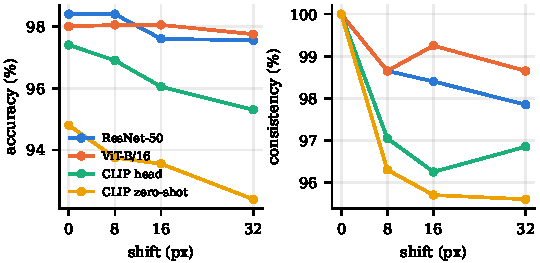
\includegraphics[width=0.49\linewidth,height=1.5in,keepaspectratio]{fig_t1_translation.pdf}\hfill
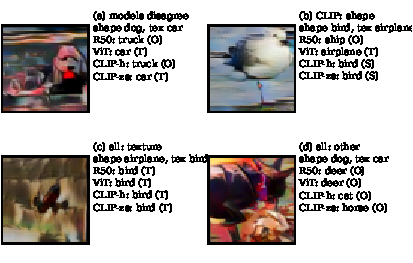
\includegraphics[width=0.49\linewidth,height=1.5in,keepaspectratio]{fig_t1_cue_examples.pdf}
\caption{\textbf{Left:} accuracy and prediction consistency as the image is shifted (average over four directions). \textbf{Right:} cue-conflict examples where (a) the models disagree, (b) only CLIP follows shape, (c) all follow texture, and (d) all pick an unrelated class. S/T/O = shape/texture/other.}
\label{fig:t1}
\end{figure}

\paragraph{Shifting is harmless, shuffling is not.} Shifting the image by 32\,px costs ResNet-50 and ViT under one point and CLIP about two, with at least 95.6\% of predictions unchanged (Fig.~\ref{fig:t1}, left). We expected the CNN to be clearly more stable here, but the ViT is just as stable. Shuffling the tiles separates the models much more. ResNet-50 loses 9.6 points, ViT only 6.0, and CLIP the most, 20.6 points with the head and 14.4 zero-shot. Even with the layout destroyed, ResNet-50 and ViT still classify 88.8\% and 92.0\% of the shuffled images correctly, so most of their decisions do not need the global arrangement of the object, and the advantage we expected from the CNN's local filters did not show up. A confident prediction is not the same as a correct one, though. When ResNet-50 gets a shuffled image wrong, it is still 68\% confident on average, and more than a quarter of these mistakes are made with over 80\% confidence.

\begin{table}[t]
\centering\small
\caption{Feature stability $I_T$ (average cosine similarity to the clean image), split by whether the prediction stayed the same ($=$) or changed ($\neq$), together with prediction consistency (\%). For cue conflict the reference is the original, unstylised image.}
\label{tab:rep}
\setlength{\tabcolsep}{2.6pt}
\begin{tabular}{l ccc ccc ccc}
\toprule
& \multicolumn{3}{c}{ResNet-50} & \multicolumn{3}{c}{ViT-B/16} & \multicolumn{3}{c}{CLIP}\\
\cmidrule(lr){2-4}\cmidrule(lr){5-7}\cmidrule(lr){8-10}
Intervention & $I_T$ & $I_T^{=}$ / $I_T^{\neq}$ & Cons. & $I_T$ & $I_T^{=}$ / $I_T^{\neq}$ & Cons. & $I_T$ & $I_T^{=}$ / $I_T^{\neq}$ & Cons.\\
\midrule
\TrepRows
\bottomrule
\end{tabular}
\end{table}

\begin{figure}[t]
\centering
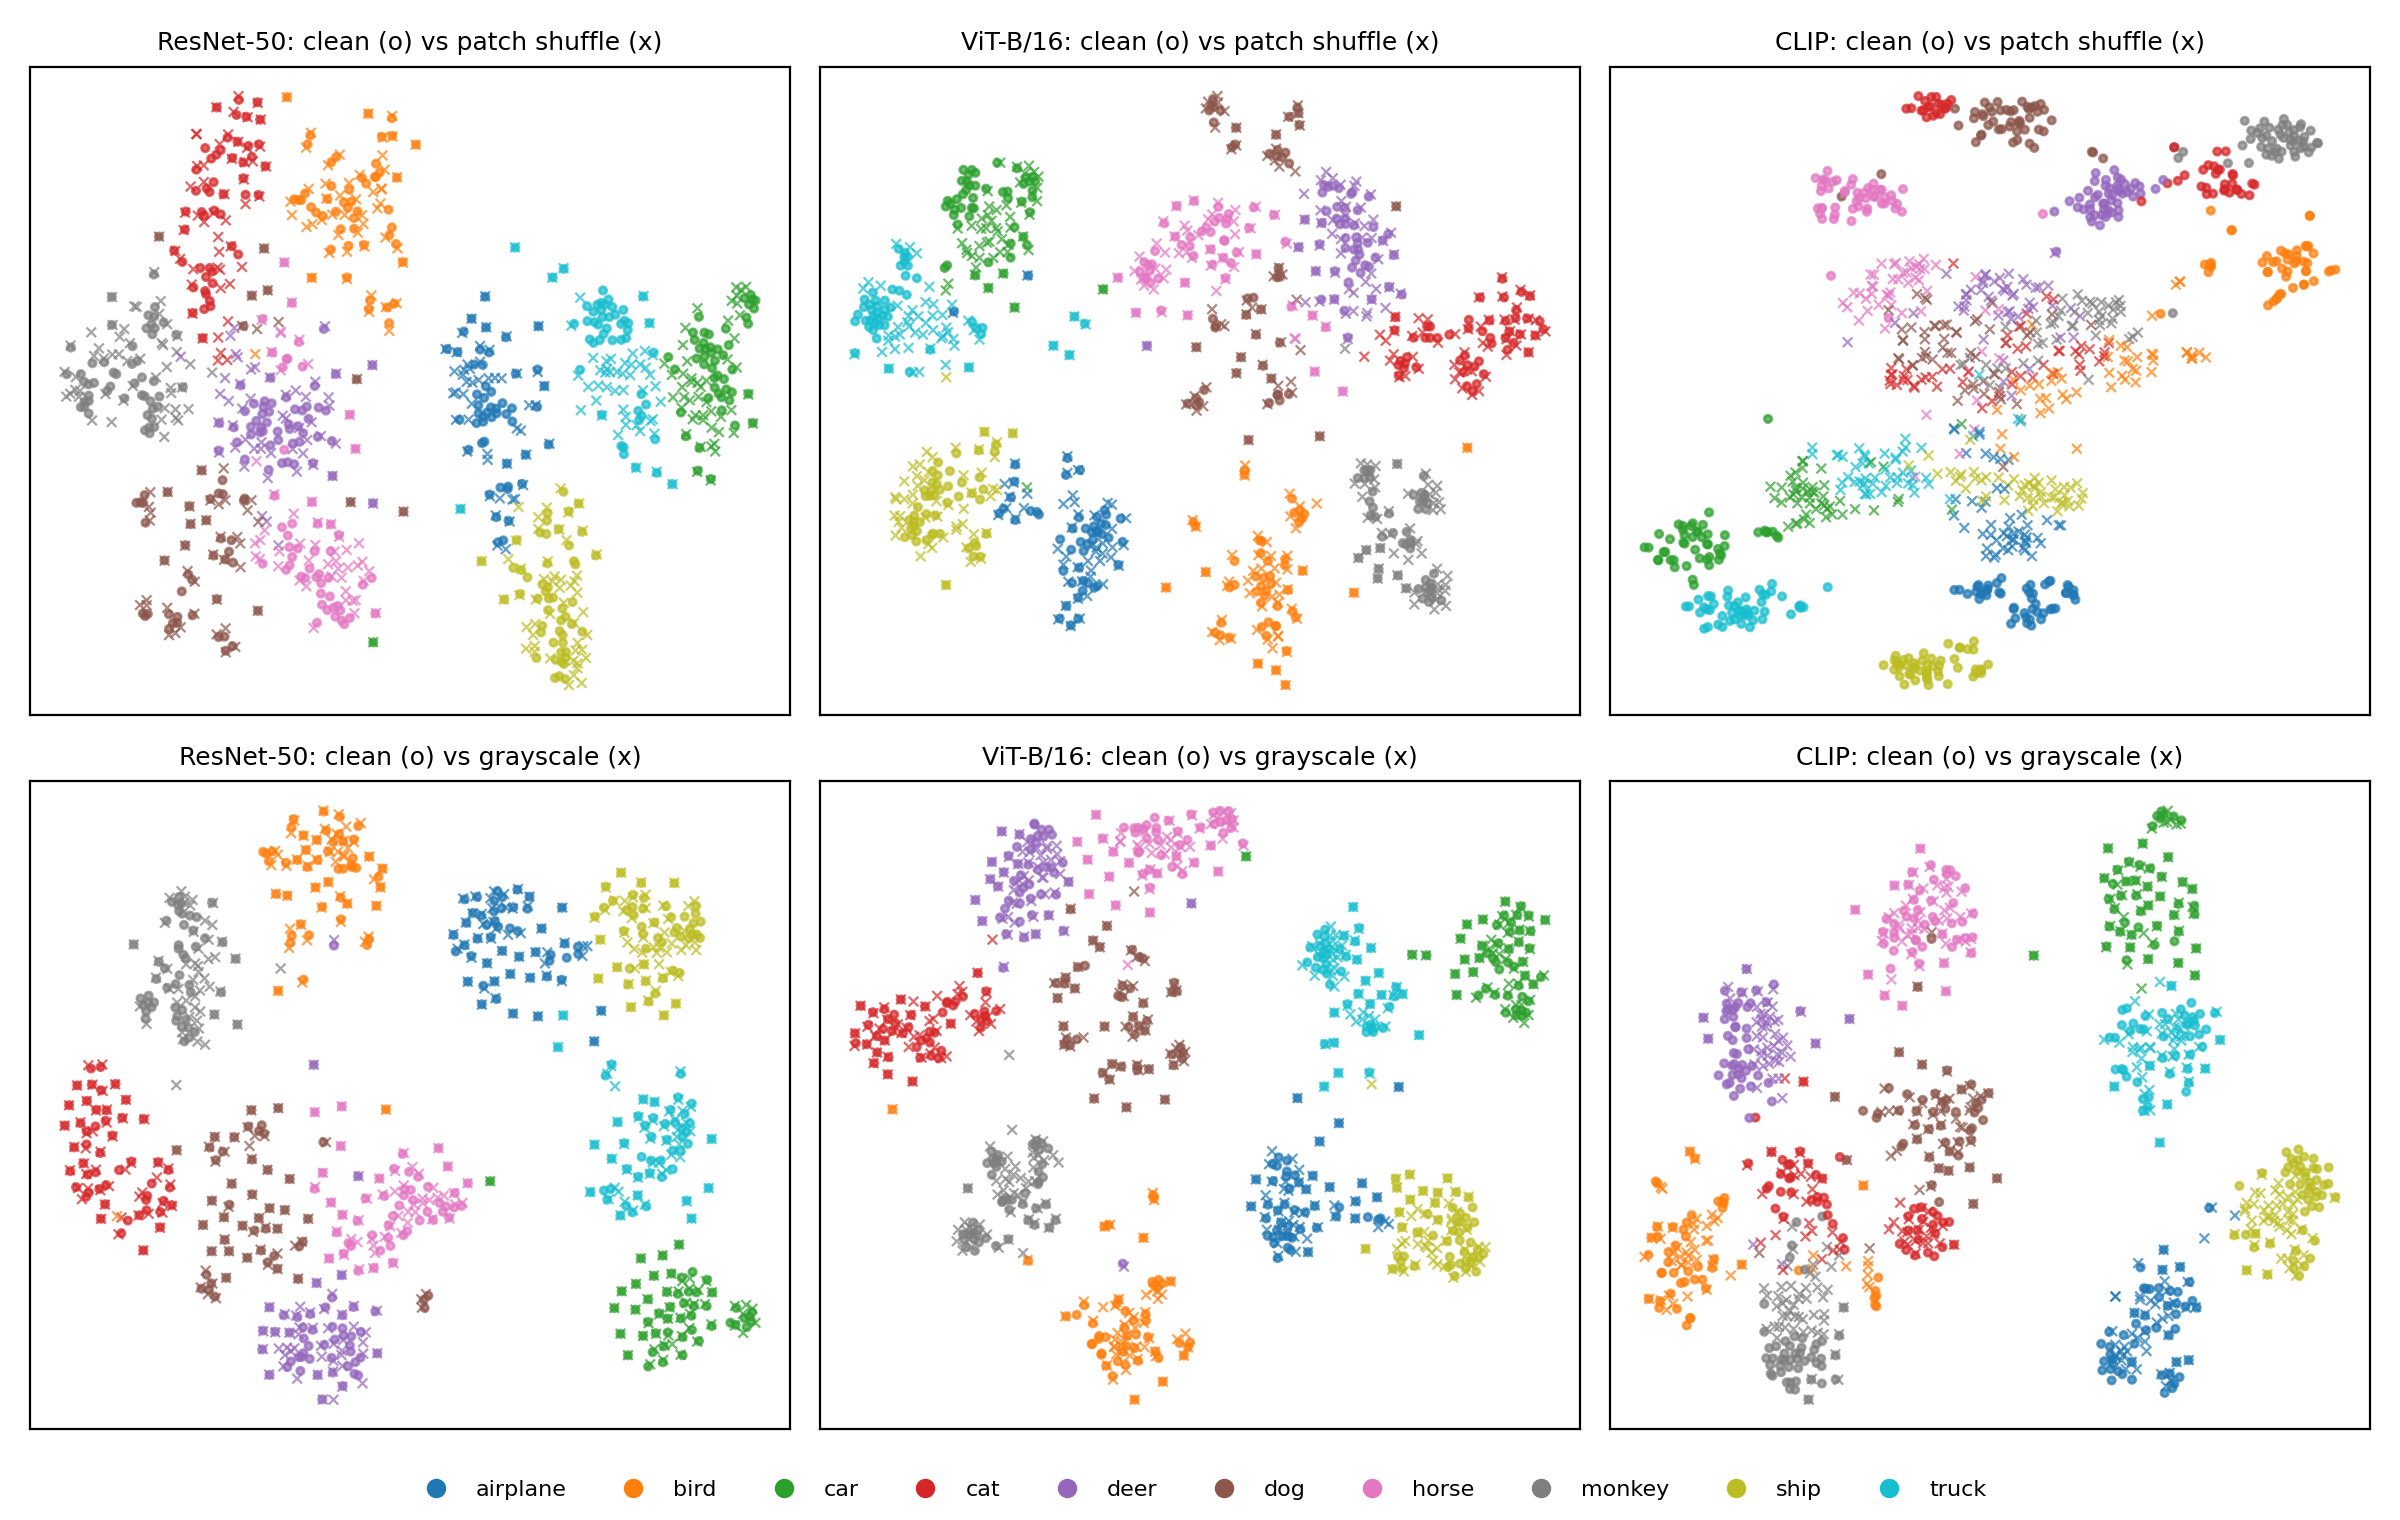
\includegraphics[width=0.48\linewidth]{fig_t1_tsne.png}
\caption{t-SNE of clean (o) and changed (x) features, fitted separately for each backbone and each change; colour shows the class.}
\label{fig:tsne}
\end{figure}

\paragraph{Do predictions and features tell the same story?} Only partly (Table~\ref{tab:rep}). Stable predictions can hide features that move quite a lot: under grayscale and hue rotation, 94 to 97\% of predictions stay the same while the ResNet and ViT features move to a similarity of 0.71 to 0.81. Even so, 95 to 97\% of these images still have their own original as the nearest clean feature, so the change is small compared with the differences between images. Where the two measures do agree is on \emph{which} images are affected: in every case, images whose prediction flipped moved further than those that didn't, and the gap is largest for cue conflict (0.47 vs.\ 0.21 for ResNet). The raw similarity values, however, can't be compared across models. CLIP has the highest similarity after shuffling (0.755), yet 23\% of its predictions flip, and only 39.6\% of shuffled images find their own original as the nearest clean feature, compared with 97.4\% for ResNet. The t-SNE plot matches this (Fig.~\ref{fig:tsne}): ResNet and ViT place shuffled images inside the clusters of their clean classes, while CLIP places them in a separate region, still grouped by class but away from the clean clusters. CLIP's two classifiers also react differently. On clean images they agree 96.6\% of the time and the trained head is slightly better (15 vs.\ 2 images that only one of them gets right), but after shuffling agreement drops to 84\% and the zero-shot classifier wins 40 to 22, even though both use exactly the same features.

\paragraph{Architecture or training data?} Our results can only partly separate the two. ResNet-50 and ViT-B/16 were trained on the same ImageNet data, so the differences between them (shape bias 69.0 vs.\ 86.8\%, shuffle loss 9.6 vs.\ 6.0 points) are the closest we get to an architecture effect, although their training recipes and sizes (about 25M vs.\ 86M parameters) also differ. CLIP and ViT are both vision transformers but were trained on different data with a different objective, and CLIP is both the \emph{most} shape-biased model (90.2\%) and the \emph{most} shuffle-sensitive one ($-20.6$ points), so for these two properties the training data and objective make at least as much difference as the architecture. Finally, the CNN and the ViT are equally stable under shifting (both lose under one point at 32\,px), so in our results translation stability is not something only the convolutional model has.

%--------------------------------------------------------------------------
\subsection{Task 2: can unlabeled sketches close the gap?}

\begin{table}[t]
\centering\small
\caption{Task 2: source-validation accuracy / macro-F1 for each source domain (\%), their average, Sketch results, change vs.\ source-only, and domain separability (50\% = chance).}
\label{tab:t2}
\setlength{\tabcolsep}{3pt}
\begin{tabular}{l ccc c cc c c}
\toprule
Method & Photo & Art & Cartoon & Mean src & Sketch acc & Sketch F1 & $\Delta$acc & Sep.\\
\midrule
Source-only & 96.1/95.6 & 92.9/93.2 & 94.2/94.6 & 94.4/94.5 & 71.0 & 71.3 & -- & 99.9\\
DAN         & 95.8/95.2 & 89.3/89.7 & 94.7/95.1 & 93.2/93.3 & \textbf{72.7} & 66.3 & $+1.7$ & \textbf{89.3}\\
DANN & 96.1/95.4 & 87.8/87.7 & 93.8/93.8 & 92.6/92.3 & 69.7 & \textbf{71.7} & $-1.3$ & 99.7\\
CDAN & 97.0/96.4 & 91.2/91.3 & 91.5/91.6 & 93.2/93.1 & 46.9 & 52.0 & $-24.1$ & 100.0\\
\bottomrule
\end{tabular}
\end{table}

\begin{figure}[t]
\centering
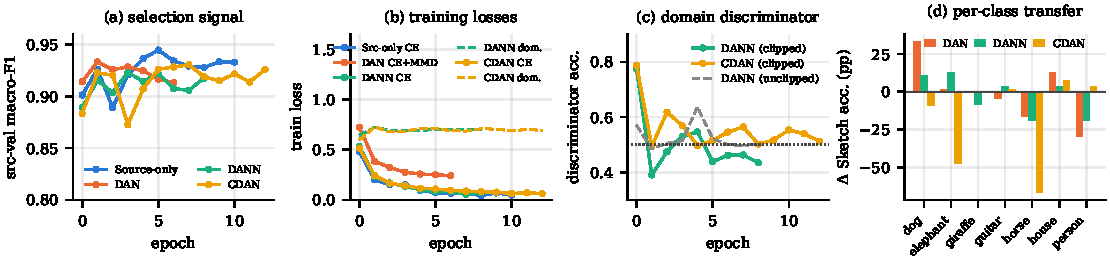
\includegraphics[width=\linewidth]{t2.pdf}
\caption{Task 2 training. (a)~Average source-validation F1, the only signal used to choose checkpoints. (b)~Training losses: classification loss for every method and the domain loss (dashed) for DANN and CDAN, which stays near $0.69$, the value expected when the domain classifier is being fooled. DAN only saved its total loss. (c)~Accuracy of the domain classifier; the unstabilised DANN only reaches 50\% because it had already broken down. (d)~Change in Sketch accuracy per class compared with source-only.}
\label{fig:t2}
\end{figure}

\paragraph{How big is the gap, and where does it come from?} The source-only model scores 94.4\% on the source domains but only 71.0\% on sketches, a drop of 23.4 points (Table~\ref{tab:t2}). Most of that loss comes from the animals. Only 24.5\% of dog sketches are recognised: 330 of the 772 are called \emph{horse} and 135 \emph{person}. Giraffes do a little better at 62.5\%, with 191 of them also called horse. Guitars, horses and people all stay above 91\%. Fig.~\ref{fig:t2}(a to c) confirms that all four methods trained properly.

\paragraph{Does making domains harder to tell apart improve recognition?} Not reliably. DAN is the only method that clearly makes the domains harder to separate (99.9 down to 89.3\%) and the only one that improves Sketch accuracy, but even its macro-F1 falls by 5 points, because the gain is very uneven (Fig.~\ref{fig:t2}d). Dogs improve by 33 points, but people lose 29 points (57 of the 160 person sketches become \emph{house}) and horses lose 17. DANN is more deceptive. Its domain classifier ends up at chance during training, which looks like success, yet a fresh classifier trained on the final features still tells the domains apart 99.7\% of the time. DANN fooled its own domain classifier without actually removing the domain information. What it did change was the class boundaries: elephants and dogs improved by 12.6 and 10.6 points, horses fell by 19.1 (180 horses are now called elephants), and overall accuracy dropped by 1.3 points.

\paragraph{Does aligning classes preserve their meaning?} In our case it did the opposite. CDAN has the best Photo accuracy (97.0\%), leaves the domains fully separable (100\%), and loses 24.1 points on sketches, because it pushes most of them into the \emph{person} class: 596 dogs, 440 elephants and 316 horses. CDAN conditions its alignment on the model's own class predictions for the sketches, and our source-only model already got three quarters of the dog sketches wrong, so aligning by those predictions did not protect the class structure here.

\paragraph{How strong should the alignment be?} We expected stronger DANN alignment to cost a little source accuracy and help on sketches up to a point, but the results look very different. With a maximum strength of 0.25 the model reaches 93.1\% on the sources but only 17.1\% on sketches; at 0.5 it gets 93.2\% and 22.7\%; and at 1.0 it gets 92.6\% and 69.7\%. Separability stays between 99.7 and 100\% in all three. Source accuracy barely moves while Sketch accuracy swings by 53 points, and the two weaker settings collapse to predicting a single class for almost every sketch (\emph{person} at 0.25, \emph{dog} at 0.5). If we had chosen the strength using the best source F1, we would have picked 0.5, the second-worst option on sketches. With one run per setting, we read this mainly as instability.

%--------------------------------------------------------------------------
\subsection{Task 3: can a model survive a domain it never sees?}

\begin{table}[t]
\centering\small
\caption{Task 3 (\%). Worst = weakest source domain. Separability is between the three sources (33\% = chance). Sharpness is the rise in loss after a small worst-case step. The last two rows are the extra DAN-DG strengths; the main comparison uses $\lambda{=}1$.}
\label{tab:t3}
\setlength{\tabcolsep}{2.8pt}
\begin{tabular}{l ccc cc cc c cc}
\toprule
Method & Photo & Art & Cartoon & Mean & Worst & Sketch acc & Sketch F1 & $\Delta$acc & Sep. & Sharp.\\
\midrule
ERM                & 96.1 & 92.9 & 94.2 & 94.4 & 92.9 & \textbf{71.0} & \textbf{71.3} & -- & 89.0 & 0.352\\
DAN-DG ($\lambda{=}1$) & 25.7 & 22.0 & 17.3 & 21.7 & 17.3 & 4.1 & 1.1 & $-66.9$ & 37.9 & 0.109\\
SAM & 98.2 & \textbf{93.9} & 95.3 & 95.8 & \textbf{93.9} & 66.4 & 69.2 & $-4.6$ & 85.4 & 0.137\\
\midrule
DAN-DG $\lambda{=}0.1$ & \textbf{98.5} & 92.4 & \textbf{96.8} & \textbf{95.9} & 92.4 & 57.3 & 58.6 & $-13.7$ & 68.1 & 0.211\\
DAN-DG $\lambda{=}10$ & 25.7 & 22.0 & 17.3 & 21.7 & 17.3 & 4.1 & 1.1 & $-66.9$ & 36.9 & 0.031\\
\bottomrule
\end{tabular}
\end{table}

\begin{figure}[t]
\centering
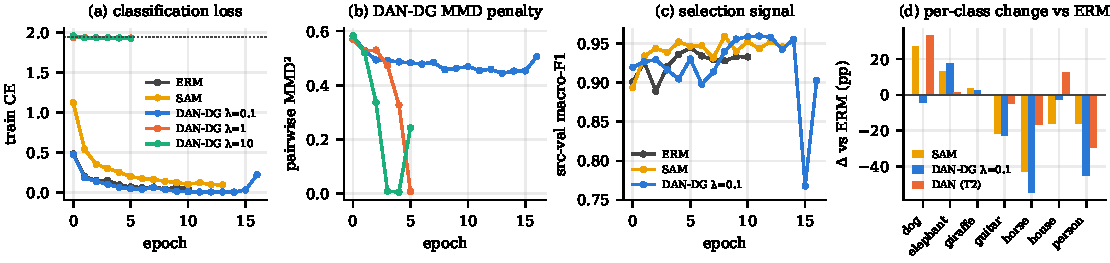
\includegraphics[width=\linewidth]{t3.pdf}
\caption{Task 3 training. (a)~Classification loss; for DAN-DG with $\lambda$ of 1 and 10 (overlapping lines) it never drops below the level of random guessing. (b)~The DAN-DG alignment penalty, which the collapsed runs push to almost zero. (c)~Average source-validation F1 for the runs that did not collapse. (d)~Change in Sketch accuracy per class compared with ERM, for SAM, DAN-DG with $\lambda{=}0.1$ and DAN from Task~2.}
\label{fig:t3}
\end{figure}

\paragraph{Do source results predict Sketch results?} No. If we rank the models by average source accuracy, DAN-DG ($\lambda{=}0.1$, 95.9\%) comes first, then SAM (95.8\%), then ERM (94.4\%). On sketches the order is exactly reversed: 57.3, 66.4 and 71.0\% (Table~\ref{tab:t3}). The weakest source domain doesn't help much either. SAM and the milder DAN-DG also train smoothly and reach a higher validation score than ERM (Fig.~\ref{fig:t3}a,c), so nothing on the source side gives a warning. The damage only shows up per class (Fig.~\ref{fig:t3}d). SAM improves dogs by 27 points and elephants by 13, but loses 43 points on horses and 22 on guitars, while DAN-DG loses 54 points on horses and 45 on people.

\paragraph{Does removing differences between the sources help?} DAN-DG does exactly what it is designed to do: the source domains become much harder to tell apart, with separability dropping from 89.0\% to 68.1\% ($\lambda{=}0.1$) and to 37.9\% ($\lambda{=}1$). Sketch accuracy, however, drops right along with it. At $\lambda$ of 1 or more the classification loss never improves from the first epoch while the alignment penalty goes to almost zero (Fig.~\ref{fig:t3}a,b), and the network predicts \emph{person} for every image, so it never learned the task at all. With $\lambda{=}0.1$ the model does learn the sources (95.9\% on average), but on sketches it loses 54 points on horses and 45 on people. In both cases, the lower the source separability, the lower the Sketch accuracy.

\paragraph{Does a flatter solution transfer better?} SAM does make the model flatter, reducing the sharpness score from 0.352 to 0.137, and it improves every source domain, but it is 4.6 points \emph{worse} on sketches. Ranked from flattest to sharpest, the models come out roughly in the reverse of their Sketch order, and the two ``flattest'' ones are the collapsed models that predict the same class for everything. In our results, a lower sharpness score did not go with better Sketch accuracy.

\paragraph{What are unlabeled sketches worth?} DAN in Task~2 and DAN-DG in Task~3 use the same alignment code with the same strength of $\lambda{=}1$. Aligning the sources with unlabeled sketches gave a gain of 1.7 points, while aligning the sources with each other collapsed the model, and even the milder setting lost 13.7 points. So with the same method and strength, having the target domain in the alignment made the difference between a small gain and a collapse. We can't attribute this to target access alone, though: the two methods also compare different numbers of images per penalty term, and each result comes from a single run.

%--------------------------------------------------------------------------
\subsection{Task 4: teaching a classifier to say ``I don't know''}

\begin{table}[t]
\centering\small
\caption{Left: four unknownness scores on the same trained model. Right: the three models compared with the MLS score, plus PROSER's own dummy-class score. FPR = \% of unknowns wrongly accepted when 95\% of known validation images are accepted. For the four scores and the MLS rows, 94.6 to 95.3\% of known CIFAR-10 test images are accepted.}
\label{tab:t4}
\setlength{\tabcolsep}{2.5pt}
\begin{tabular}{l ccc cc}
\toprule
\multicolumn{6}{c}{\emph{Scores (Vanilla, accuracy 94.8\%)}}\\
Score & \multicolumn{3}{c}{AUROC near / far / all} & \multicolumn{2}{c}{FPR near / far}\\
\midrule
MSP  & \multicolumn{3}{c}{\textbf{.812} / .901 / .856} & \multicolumn{2}{c}{72.5 / 57.4}\\
MLS  & \multicolumn{3}{c}{.795 / .894 / .844} & \multicolumn{2}{c}{\textbf{65.4} / 47.1}\\
Energy & \multicolumn{3}{c}{.795 / .894 / .845} & \multicolumn{2}{c}{66.4 / \textbf{46.6}}\\
Mahalanobis & \multicolumn{3}{c}{.798 / \textbf{.919} / \textbf{.858}} & \multicolumn{2}{c}{72.8 / 50.5}\\
\bottomrule
\end{tabular}\hfill
\begin{tabular}{l c ccc cc}
\toprule
\multicolumn{7}{c}{\emph{Models (score = MLS unless noted)}}\\
Model & Acc. & \multicolumn{3}{c}{AUROC n / f / all} & \multicolumn{2}{c}{FPR n / f}\\
\midrule
Vanilla & 94.8 & .795 & .894 & .844 & 65.4 & 47.1\\
GCSC    & \textbf{95.3} & \textbf{.811} & \textbf{.895} & \textbf{.853} & \textbf{63.8} & \textbf{40.4}\\
PROSER  & 94.1 & .782 & .854 & .818 & 70.1 & 57.1\\
PROSER (dummy) & 94.1 & .779 & .886 & .833 & 71.1 & 51.0\\
\bottomrule
\end{tabular}
\end{table}

\begin{figure}[t]
\centering
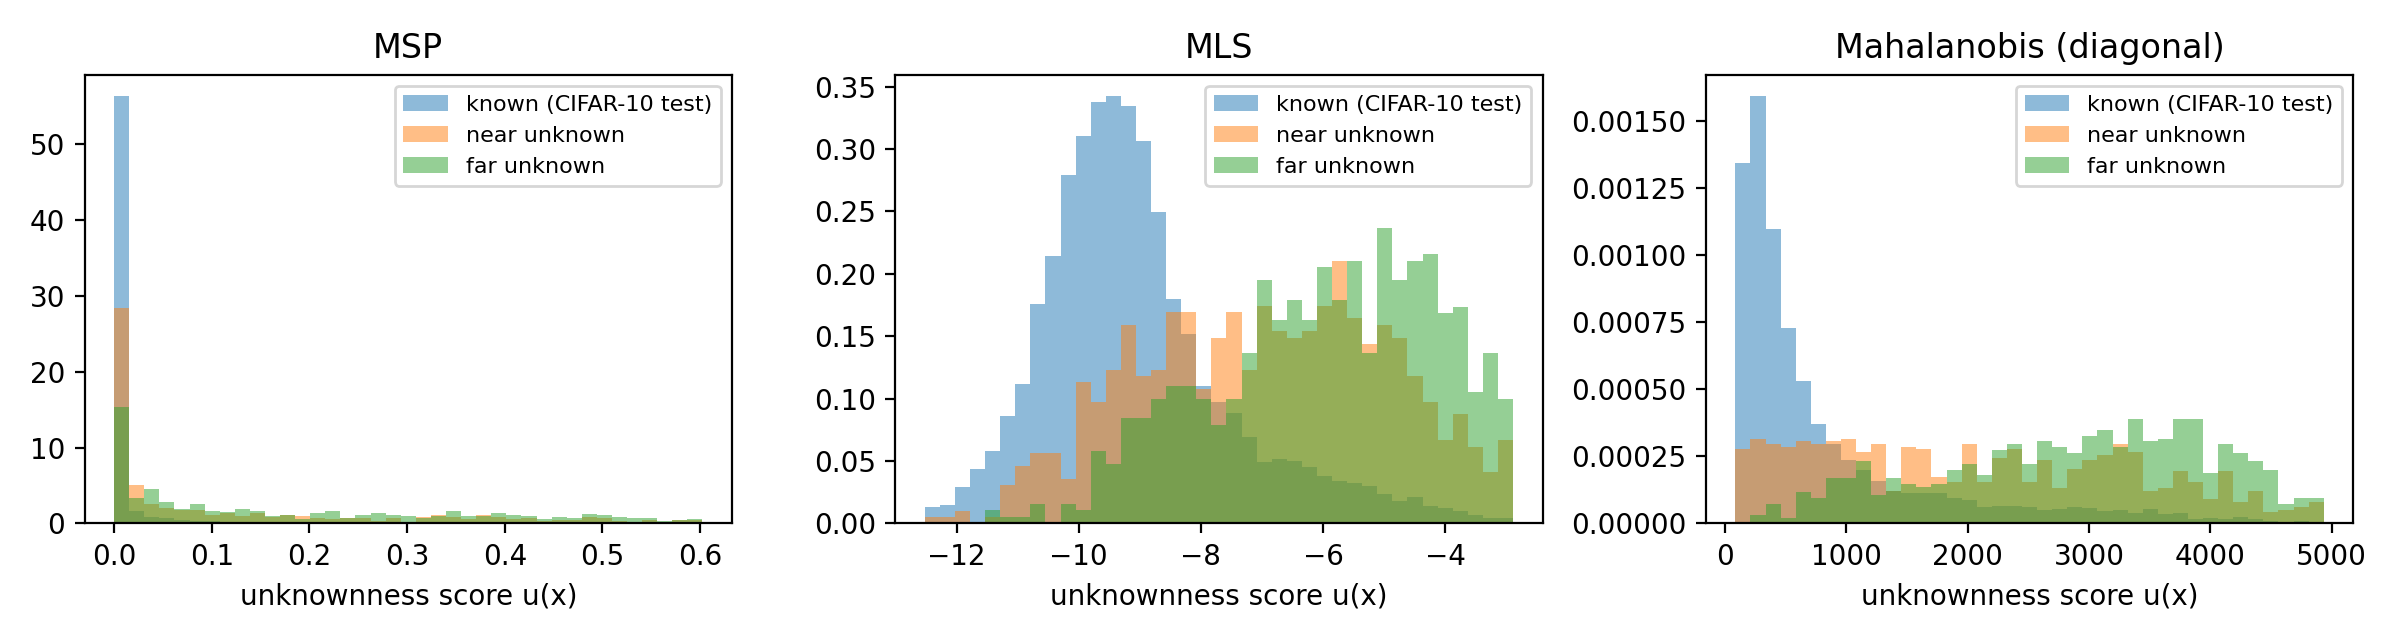
\includegraphics[width=0.7\linewidth]{score_distributions.png}
\caption{Unknownness scores on the Vanilla model for known test images and near and far unknowns. With MLS the near unknowns overlap the known images, while the far ones sit further right. With Mahalanobis distance, far unknowns spread far to the right, but many near unknowns sit as close to the class centres as known images.}
\label{fig:t4}
\end{figure}

\paragraph{How does similarity to known classes affect rejection?} Near unknowns are much harder to reject. With the MLS score, 65.4\% of them are accepted as known, compared with 47.1\% of the far ones (Table~\ref{tab:t4}). The classes that slip through most often are the ones closest in meaning to a CIFAR-10 class, and each is absorbed by that class: 84\% of pickup trucks are accepted (mostly as automobiles or trucks), 82\% of buses (mostly as trucks) and 76\% of wolves (as dogs or cats). Motorcycles are rejected most often among the near classes, with only 42\% accepted. Among the far classes, wardrobes (71\% accepted) and sunflowers (56\%, mostly as birds) were the surprises. The most confident mistakes also split into sensible and strange ones. For near unknowns they are a bus taken for a truck and two camels taken for deer, while for far unknowns they are a keyboard taken for a truck, a chair taken for an airplane and a bowl taken for a cat. All six scored as more ``known'' than a typical correctly classified CIFAR-10 image.

\paragraph{What does each score capture?} Plain softmax confidence (MSP) is the best at ranking near unknowns. MLS and energy behave almost identically (their rankings match perfectly, Spearman 1.00). At the actual decision threshold, however, MLS and energy accept fewer near unknowns than MSP (65.4 vs.\ 72.5\%), even though MSP ranks them better overall, which shows that AUROC and a fixed threshold measure different things. Mahalanobis distance looks at the features rather than the outputs, and it disagrees with MLS in a telling way. On near unknowns, MLS rejects 86 images that Mahalanobis accepts, while only 27 go the other way. On far unknowns the two are much more balanced (107 vs.\ 80), and rejecting an image when \emph{either} score flags it would catch 63\% of far unknowns instead of 53\% with MLS alone, but only 38\% instead of 35\% of near ones. In our results, the output-based scores are better on near unknowns, while feature distance is the best score on far unknowns (AUROC .919).

\paragraph{Does stronger augmentation help?} Yes, on both counts. Adding RandAugment (GCSC) raises test accuracy by half a point and improves every MLS measure, most of all the share of far unknowns wrongly accepted, which drops from 47.1 to 40.4\%. The improvement is uneven, though: near unknowns improve much less (65.4 to 63.8\% accepted), and with the Mahalanobis score GCSC's near-unknown result even gets worse (AUROC .798 to .764).

\paragraph{Do the dummy classes (PROSER) help?} Not in our runs. The MLS AUROC fell from .844 to .818, PROSER's own dummy-class score recovered only part of that (.833), and test accuracy dropped by 0.7 points. The training log shows that validation accuracy peaked after the first epoch of fine-tuning (94.6\%, the checkpoint we kept) and then settled around 91\% as the dummy-class losses fell to about 0.02, so the dummy-class training cost known-class accuracy. It did not buy better rejection of near unknowns either (70.1\% accepted, vs.\ 65.4\% for Vanilla), even though the dummy classes are trained on mixtures of known classes. Overall, improving the classifier itself (GCSC) did more for rejecting unknowns than training it on made-up ones.

%==========================================================================
\section{Cross-task discussion}\label{sec:disc}
\paragraph{Visual cues and domain shift.} Task~1 and the PACS results point in the same direction. In Task~1, removing colour changed at most 5.2\% of predictions, while texture conflicts often decided ResNet-50's answer. On PACS, the sketches have neither colour nor photo-like texture, and the source-only ResNet-18's biggest failures are four-legged animals (330 dogs and 191 giraffes called horses), while classes with more distinctive outlines transfer well, such as guitars (93.6\%) and houses (87.5\%). This is consistent with texture, rather than colour, being the cue that goes missing on sketches, but the two tasks use different datasets and networks, so we cannot test that link directly.

\paragraph{Invariance versus keeping the label.} Across Tasks 2 and 3, making the domains harder to tell apart came with better target accuracy only once (DAN, and even then macro-F1 fell). Every other large drop in separability came either from a collapsed model (DAN-DG with $\lambda$ of 1 or more) or from large losses on specific classes (DAN-DG with $\lambda{=}0.1$ lost 54 points on horses and 45 on people). In our results, low domain separability on its own was not a sign of a better model, and was often a sign of a broken one; it only becomes meaningful when read together with class accuracy.

\paragraph{The value of target data.} With the same alignment code and strength, including unlabeled sketches (DAN) gave the only positive transfer in the study, while aligning only the sources (DAN-DG) collapsed the model.

\paragraph{Recognising versus rejecting.} In Task~4 the best ordinary classifier was also the best at rejecting unknowns (GCSC), and the method built for rejection (PROSER) was worse at both. Yet every model still accepted 64 to 71\% of near unknowns, much like Task~1's shuffled images still received confident labels. The accepted near unknowns are mostly absorbed by their closest known class (wolf to dog or cat, bus to truck), and no model or score we tested rejected more than 36.3\% of them at the chosen threshold.

\paragraph{So what should a robust representation do?} Based on our results, it should \emph{keep} shape information: the most shape-biased model (CLIP) followed shape on 90 to 93\% of cue conflicts, and on sketches the classes with distinctive outlines transferred best. It should \emph{learn to ignore} domain differences only when there is evidence about the target: alignment with unlabeled sketches helped slightly, while alignment among the sources alone lowered Sketch accuracy along with domain separability. And it should \emph{refuse} inputs more often than a plain classifier does, since even the best model accepted about two thirds of near unknowns with scores calibrated on known data.

\section{Conclusion}
Every intuitive sign of robustness fooled us at least once: stable predictions, domains that are hard to tell apart, flat minima, high source accuracy and made-up unknowns. Each time, a class-by-class look at the failures was needed to tell a real improvement from a collapse or a reshuffling of classes. The main limitations are single runs, the stability fix for the adversarial methods, one style-transfer strength and a single-batch sharpness score.

\end{document}
